% ============================================================================
%  Chapter 5 — Layered Defenses and Two-Instrument Measurement
%  Thesis: Generative AI, Privacy & Personal Data — TADJ Mohamed Walid, ESI SBA
%
%  DUAL-MODE FILE. Compiles standalone (for drafting) AND is \input-able into a
%  future thesis.tex. When the master document defines \ThesisMaster before
%  \input, the standalone preamble below is skipped.
%
%  CITATIONS: \cite{...-TODO} are placeholders. The unified .bib is separate
%  scaffolding work (PHASE5_PLAN.md §4.2), not part of this chapter task.
%
%  NUMBERS: every figure traces to a committed artifact. Ablation / kappa / bounds
%  values are from results/phase3/ablation/metrics/final_metrics.json,
%  results/phase3_4/judge_defended_calibration/kappa_defended.json, and
%  .../residual_bounds.json. The oracle (0.933->0.000), sanitized-corpus (87%),
%  and layer-validation counts are consolidated from the committed, supervisor-
%  reviewed Phase3_4_Report_Expanded.tex (§4); their upstream data home is
%  results/retrieval_conditional/ and the sanitize/guard logs (cite for final).
% ============================================================================
\ifdefined\ThesisMaster\else
  \documentclass[11pt,a4paper]{report}
  \usepackage[utf8]{inputenc}
  \usepackage[T1]{fontenc}
  \usepackage{lmodern}
  \usepackage[margin=2.5cm]{geometry}
  \usepackage{booktabs}
  \usepackage{tabularx}
  \usepackage{amsmath,amssymb}
  \usepackage{graphicx}
  \usepackage{microtype}
  \usepackage{xcolor}
  \usepackage[hidelinks]{hyperref}
  \graphicspath{{../}{../../../phase3/ablation/metrics/}{../../../phase3/report/}}
  \begin{document}
\fi

\chapter{Layered Defenses and Two-Instrument Measurement}
\label{ch:defenses}

This chapter assembles the privacy defenses into a single layered stack, measures how
much of the baseline leakage they remove, and asks whether the instrument used to measure
that removal can itself be trusted. These are the two empirical questions at the center of
the thesis. \textbf{RQ2} asks how much existing defense mechanisms actually reduce measured
leakage; \textbf{RQ3} asks whether a language-model judge can detect and classify that
leakage with calibrated confidence and a bounded false-positive rate. The two questions are
inseparable, because the answer to RQ2 depends on which instrument does the measuring. The
central result of the chapter is that the two natural instruments, a deterministic rule engine and
a validated language-model judge, disagree systematically and in opposite directions on exactly
the redacted and refused output the defenses produce. That disagreement is not noise to be
averaged away; it is itself the finding. The measured leakage rate of a defended
retrieval-augmented system is instrument-dependent, and a single number from a single instrument
conceals more than it reveals.

The chapter is, throughout, a \emph{demonstration} of how to measure a defended system honestly on
a controlled corpus, not a certification that the resulting system is safe to deploy. The numbers
below are exact for this corpus and these scenarios; their value is the method and the relative
findings they establish, not an absolute guarantee.

\section{The layered defense}
\label{sec:ch5-defense}

The defense composes five mechanisms (\Cref{fig:ch5-pipeline}), each closing a distinct path by which personal data
escapes a retrieval-augmented pipeline. An \emph{input filter} blocks injection and
jailbreak attempts before they reach retrieval, so an adversarial instruction never enters
the system. \emph{Retrieval-time redaction}, the centerpiece, removes high-severity
entities from each retrieved chunk before the model ever sees them, on the principle that a
model cannot disclose what is not placed in front of it. A \emph{conversation-aware} layer
refuses when the facts accumulated about a single individual across a dialogue cross a
threshold, catching the gradual disclosure that any per-response check misses. An
\emph{output filter} redacts the response itself, catching identifiers the model surfaces
or reformats. Finally, a \emph{provenance} layer quarantines any retrieved document absent
from a trusted list, defeating corpus poisoning. Each mechanism was validated against a
real attack rather than asserted in principle (Table~\ref{tab:ch5-layers}).

\begin{table}[h]
\centering
\caption{The five defense mechanisms: where each acts, what it does, and the attack it was
validated against.}
\label{tab:ch5-layers}
\begin{tabularx}{\textwidth}{lp{2.6cm}X}
\toprule
\textbf{Mechanism} & \textbf{Where it acts} & \textbf{What it does, and how it was validated}\\
\midrule
Input filter & before retrieval & Blocks injection and jailbreak attempts: 2/2 attacks blocked, 0/3 benign queries wrongly blocked; no model call once an attempt is rejected.\\
Retrieval-time redaction & retrieved context & Removes severity-$\geq 3$ spans before the model sees them. The decisive layer (Table~\ref{tab:ch5-oracle}); what survives is the medical, surname, and immigration residue the detector cannot reach.\\
Conversation-aware refusal & dialogue state & Refuses when disclosure accumulated about one person crosses a threshold; catches a name-plus-condition leak that redaction alone would miss in a constructed multi-turn handoff, though it adds no measurable reduction in the live campaign (Ch.~\ref{ch:tradeoff}); 0/3 false positives.\\
Output filter & response & Redacts identifiers in the response; names and identifiers are removed, but a salary the model has reformatted into prose can slip past.\\
Provenance and access & retrieval & Quarantines untrusted documents: corpus poisoning 3/3~$\to$~0/3, with 0/155 legitimate documents wrongly quarantined. Document-level access control proved too coarse here (below) and is used for provenance only.\\
\bottomrule
\end{tabularx}
\end{table}

\begin{figure}[h]
\centering
\resizebox{\textwidth}{!}{%
\begin{tikzpicture}[font=\footnotesize,
  stage/.style={draw=esidark, fill=white, rounded corners=2pt, minimum height=10mm, minimum width=16mm, align=center},
  layer/.style={draw=esiblue, fill=esiblue!12, rounded corners=2pt, minimum height=10mm, minimum width=14mm, align=center, text=esiblue},
  arr/.style={-{Latex[length=2mm]}, esidark, semithick}]
\node[stage] (q) {User\\query};
\node[layer, right=3.5mm of q] (l1) {\textbf{L1}\\input};
\node[stage, right=3.5mm of l1] (ret) {Retriever\\ChromaDB\\$k{=}5$};
\node[layer, right=3.5mm of ret] (l5) {\textbf{L5}\\prov.\,/\,ACL};
\node[layer, right=3.5mm of l5] (l2) {\textbf{L2}\\redact};
\node[stage, right=3.5mm of l2] (llm) {LLM\\Sonnet\,4.6};
\node[layer, right=3.5mm of llm] (l3) {\textbf{L3}\\refuse};
\node[layer, right=3.5mm of l3] (l4) {\textbf{L4}\\output};
\node[stage, right=3.5mm of l4] (resp) {Response};
\draw[arr](q)--(l1);\draw[arr](l1)--(ret);\draw[arr](ret)--(l5);\draw[arr](l5)--(l2);\draw[arr](l2)--(llm);\draw[arr](llm)--(l3);\draw[arr](l3)--(l4);\draw[arr](l4)--(resp);
\end{tikzpicture}}
\caption[The layered defense pipeline]{The layered defense pipeline. Pipeline stages (white)
interleave with the five defense layers (blue): \textbf{L1} input filter before retrieval;
\textbf{L5} provenance/access and \textbf{L2} retrieval-time redaction on the retrieved context;
\textbf{L3} conversation-aware refusal and \textbf{L4} output filter around generation. The
configuration encoding $\mathrm{C}[\mathrm{L1\,L2\,L3\,L4\,L5}]$ toggles each layer independently
(Table~\ref{tab:ch5-layers}).}
\label{fig:ch5-pipeline}
\end{figure}

The single most important test in the study isolates retrieval-time redaction. To remove
the variability of retrieval itself, we force the target document into the model's context
and ask directly for its sensitive contents. Without redaction the model discloses that
content almost every time; with it, disclosure collapses to nothing
(Table~\ref{tab:ch5-oracle}). What remains in the redacted context is precisely the
medical, surname, and immigration material that the detector cannot recognize: present in
the context, but not volunteered in the response, and handed to the conversation-aware
layer to refuse.

\begin{table}[h]
\centering
\caption[Retrieval-time redaction with the target document forced into context]{Retrieval-time redaction with the target document forced into context. The
disclosure rate is the fraction of trials in which the model reveals the protected content.}
\label{tab:ch5-oracle}
\begin{tabular}{lccp{5.8cm}}
\toprule
\textbf{Redaction} & \textbf{Disclosure rate} & \textbf{Trials} & \textbf{What survives}\\
\midrule
Off & 0.933 & 14/15 & everything\\
On & \textbf{0.000} & 0/15 & only medical, surname, and immigration data\\
\bottomrule
\end{tabular}
\end{table}

A preventive variant complements live redaction by sanitizing the corpus \emph{before} it
is ever indexed, so that sensitive content cannot be retrieved under any query. Applied to
the full corpus it removes 87.0\% of high-severity entities (1296 of 1490) and every hard
identifier (national identifiers, IBANs, secrets, e-mail, phone, date of birth), leaving
exactly the open-vocabulary residue the detector cannot reach: 194 entities, comprising 93
medical conditions, 49 titled surnames, 36 immigration phrases, five fragments of embedded
system text, and eleven atypically formatted addresses.

Building the stack surfaced three limitations that govern how the later numbers must be
read, and which are stated here rather than deferred. First, the rule engine credits a leak
only to entities annotated on a \emph{retrieved} document; when a response surfaces a name
and salary that live on a record the retriever did not fetch, the engine scores no leak. The
baseline figure is, for this reason, a conservative floor rather than a ceiling. Second,
output filtering is strictly weaker than input redaction for the same entity: a salary
figure the detector catches in the stored document slips past once the model has reformatted
it into prose. Third, document-level access control is too coarse for this corpus: every
legitimate document carries some high-severity content, so filtering by clearance blocks all
retrieval for lower-privilege users rather than discriminating usefully. This is why
entity-level redaction, not access control, is the right instrument here, and why the access
layer is retained for provenance alone.

\section{What redaction cannot reach: the detection ceiling}
\label{sec:ch5-ceiling}

Two of the layers above, retrieval-time redaction and the output filter, can only remove
what a PII detector first flags, so the effectiveness of the decisive layer is bounded by the
detector's recall. That ceiling was measured before the layers were built, and it governs how
the later results must be read. Of the thirty-one entity types present in the corpus, an
off-the-shelf detector recognizes only six out of the box (535 entities); four more are caught
partially, three require a custom recognizer for the corpus's national-identifier formats, and
eighteen (salaries, ages, project names, embedded secrets) are not classical patterns at
all. Equipping the detector with legitimate custom recognizers, for structured identifier
formats rather than gazetteers seeded with the corpus's own values (which would be circular),
lifts its recall on high-severity entities from $0.666$ to $0.835$. That is a real
improvement, but it falls short of the $0.90$ a single filter would have to clear before it
could be trusted to stand alone, and thirteen entity types remain below that line.

The shortfall is not spread evenly; it concentrates in a small set of categories that a
pattern-and-name detector is structurally unable to recognize (Table~\ref{tab:ch5-ceiling}).
Open-vocabulary medical conditions (93 entities, recall $0.00$) and immigration phrasing
(36 entities, $0.00$) are missed entirely, because they are clinical and legal language rather
than identifiers; half of the titled surnames slip past ($0.51$); and, most consequentially
for what follows, the combination of age and gender is missed completely (100 entities,
$0.00$): individually a low-severity attribute, but the bridge that turns scattered facts into
a re-identification.

\begin{table}[h]
\centering
\caption[Where high-severity detection fails]{Where high-severity detection fails. These categories are why a single filter cannot
suffice.}
\label{tab:ch5-ceiling}
\begin{tabular}{lccp{6.2cm}}
\toprule
\textbf{Category} & \textbf{Entities} & \textbf{Recall} & \textbf{Why it is missed}\\
\midrule
Medical conditions & 93 & 0.00 & Open clinical vocabulary; needs a trained model, not a pattern\\
Titled surnames & 100 & 0.51 & Name variants the recognizer does not generalize to\\
Immigration status & 36 & 0.00 & Open-vocabulary phrasing\\
Street addresses & 100 & 0.89 & Mostly caught; some formats slip through\\
Embedded system text & 5 & 0.00 & Semantic content, not an identifier\\
Age and gender & 100 & 0.00 & Stored form differs from the answer-key text; the linkage bridge\\
\bottomrule
\end{tabular}
\end{table}

This is the empirical case for layering, and it is also the mechanism behind
the chapter's central residual. A defense resting on a single detector inherits that
detector's ceiling. The entities left exposed are precisely the medical, surname, immigration,
and age--gender attributes from which an individual can be reconstructed across documents;
because the detector cannot flag them, redaction cannot remove them, and no downstream layer
can redact what was never marked. The cross-document linkability that
Sections~\ref{sec:ch5-rq2} and~\ref{sec:ch5-disagreement} report as the principal unreduced
residual is, at bottom, this detection ceiling expressed at the level of an attack family: not
a failure of the redaction layer, but the boundary of what any redaction layer built on this
detector could ever reach.

\section{Two instruments, and why two are needed}
\label{sec:ch5-instruments}

\begin{figure}[h]
\centering
\includegraphics[width=0.82\textwidth]{fig5_severity_distribution}
\caption[Turn-level leak counts by maximum disclosed-entity severity]{Turn-level leak counts by
maximum disclosed-entity severity for the three labeller signals. The engine fires on severity-2
entities in $66\%$ of its $L=1$ turns ($63/95$); the judge fires on severity-2 in only $2\%$
($1/57$). The augmented severity-3 and severity-4 columns are driven entirely by the judge
signal --- the empirical signature of the engine's severity-2 false-positive class.}
\label{fig:ch5-severity}
\end{figure}

Every configuration is scored twice, by two independent instruments, and the reason is
methodological rather than ornamental. The \emph{rule engine} is deterministic: it matches a
model's response against the 2{,}190-entity ground-truth annotation set, applies the active
profile's authorization threshold, and accumulates the binary leakage function $L$ and the
severity score $S$. It detects what is annotated and syntactically present. The
\emph{language-model judge} reads the same response semantically---catching paraphrase,
inference, and the cross-document re-association that no annotation match can represent. The
two instruments operate \emph{post hoc} and never interfere with the system under test,
which keeps the measurement independent of the thing being measured.

The instruments answer the same question with different sensory organs (\Cref{fig:ch5-severity}), and the difference
is visible from the very first row of results: at the undefended baseline, the engine reports
an attack-success rate of $0.192$ while the judge reports $0.288$. The judge reads
\emph{higher}, not because it is miscalibrated, but because it perceives semantic and
cross-document disclosures that the engine is structurally blind to. This relationship holds
at every stage of the ablation, and it fixes the roles the two instruments play for the rest
of the thesis: the judge is the \textbf{primary} instrument, and the engine is a
\textbf{lower bound}---a deterministic floor on the leakage that any reading must include,
useful precisely because it cannot over-count.

\section{RQ2: how much the defenses reduce leakage}
\label{sec:ch5-rq2}

\begin{figure}[h]
\centering
\begin{tikzpicture}
\begin{axis}[
  ybar, bar width=22pt, width=0.95\textwidth, height=7.4cm,
  ymin=0, ymax=34, ylabel={Strict attack-success rate (\%)}, ylabel style={font=\small},
  symbolic x coords={C00000,C01100,C11111},
  xticklabels={C00000\\\footnotesize undefended,C01100\\\footnotesize knee (L2+L3),C11111\\\footnotesize full stack},
  xtick=data, x tick label style={align=center, font=\small},
  ytick={0,5,10,15,20,25,30}, ymajorgrids, grid style={gray!15, thin},
  nodes near coords, nodes near coords style={font=\footnotesize\bfseries, /pgf/number format/fixed, /pgf/number format/precision=1},
  legend style={at={(0.5,1.05)}, anchor=south, legend columns=2, font=\small, draw=gray!35, rounded corners=2pt},
  enlarge x limits=0.35, axis line style={gray!55}, tick style={gray!55},
]
\addplot[fill=figamber, draw=figamber!60!black, line width=0.5pt] coordinates {(C00000,19.2)(C01100,1.9)(C11111,0.0)};
\addplot[fill=figblue, draw=figblue!60!black, line width=0.5pt] coordinates {(C00000,28.8)(C01100,19.2)(C11111,17.3)};
\legend{Engine (lower bound), Judge (primary)}
\end{axis}
\end{tikzpicture}
\caption[Leakage reduction across configurations, read through both instruments]{Strict
attack-success rate across three configurations, by instrument. The judge (primary) shows leakage
falling from $28.8\%$ undefended to $19.2\%$ at the redaction-plus-refusal knee (C01100) and
$17.3\%$ at the full stack --- a partial reduction of about forty percent, not an elimination.
The engine reads the same defenses as near-total ($19.2\%\!\to\!0.0\%$); the gap between the two
readings is the methodological finding of Section~\ref{sec:ch5-disagreement}, not measurement
error.}
\label{fig:ch5-reduction}
\end{figure}

With the stack assembled, six configurations were measured across the full campaign: the
undefended baseline, each of the three most informative layers in isolation, the pairing of
redaction with conversational refusal, and the complete stack, each scored through
both instruments (Table~\ref{tab:ch5-headline}). RQ2 is answered here through the binary
leakage function $L$, reported as attack-success rate; the severity-weighted reduction
$\Delta S$, which the formal framework of Chapter~\ref{ch:formal} also defines, is developed
in Chapter~\ref{ch:tradeoff} alongside the residual-risk analysis, where severity governs
the stratification.

\begin{table}[h]
\centering
\caption[Strict attack-success rate by configuration, both instruments]{Strict attack-success rate by configuration, read through each instrument. The
judged figures are primary; the engine figures are a lower bound.}
\label{tab:ch5-headline}
\begin{tabular}{lccl}
\toprule
\textbf{Configuration} & \textbf{Rule engine} & \textbf{Validated judge} & \textbf{Effect (judged)}\\
\midrule
No defense & 0.192 & \textbf{0.288} & ---\\
Input filter only & 0.231 & 0.365 & within noise\\
Retrieval redaction only & 0.019 & \textbf{0.192} & reduces leakage\\
Conversational refusal only & 0.192 & 0.346 & within noise\\
Redaction + refusal & 0.019 & 0.192 & reduces leakage\\
Full stack & 0.000 & \textbf{0.173} & reduces leakage\\
\bottomrule
\end{tabular}
\end{table}

Read through the judge, the primary instrument, the full stack reduces leakage from
$28.8\%$ to $17.3\%$, a reduction of roughly forty percent (\Cref{fig:ch5-reduction}). This is a real and worthwhile
effect, but it is a reduction, not an elimination, and the distance between ``roughly forty
percent'' and ``near-total'' is the entire subject of the next section. The reduction is not
distributed evenly across the layers. Measured against an empirically calibrated noise floor
of $0.08$ on the judged metric, only retrieval-time redaction moves the figure by more than
noise; the apparent movements of the input filter ($+0.077$) and the conversational layer
($+0.058$) sit within the floor (Table~\ref{tab:ch5-marginal}, \Cref{fig:ch5-marginal}). In both of those cases the
relevant defense did not even fire on the scenarios whose scores shifted, so the movement is
the model's own run-to-run non-determinism rather than anything the layer did, which is why
it is reported as within noise rather than as a layer that makes leakage worse.

\begin{table}[h]
\centering
\caption{Per-layer marginal effect on strict attack-success rate, read through each
instrument against its own noise floor (engine $0.04$, judged $0.08$).}
\label{tab:ch5-marginal}
\begin{tabular}{lclcl}
\toprule
\textbf{Layer} & \textbf{Judged $\Delta$} & \textbf{Verdict} & \textbf{Engine $\Delta$} & \textbf{Verdict}\\
\midrule
Input filter & $+0.077$ & within noise & $+0.039$ & within noise\\
Retrieval redaction & $-0.096$ & reduces leakage & $-0.173$ & reduces leakage\\
Conversational refusal & $+0.058$ & within noise & $+0.000$ & within noise\\
\bottomrule
\end{tabular}
\end{table}

This is not the claim that only one layer works. The input filter blocks attacks
that carry no high-severity payload and therefore cannot register on a leakage metric at all;
the conversational layer defends an axis (disclosure accumulated across dialogue turns) that
this single-pass metric barely exercises; the provenance layer defeats poisoning outright.
Each protects against something this particular measurement does not score. What the
measurement \emph{does} establish is that retrieval-time redaction is the layer that reduces
personal-data leakage, and that adding the remaining layers on top of redaction-plus-refusal
buys no further reduction the instrument can distinguish from noise. The practical
consequence is a deployment ``knee'': the redaction-plus-refusal pair (configuration C01100)
reaches a judged rate of $0.192$, and the full stack's additional descent to $0.173$ is a gap
of $0.019$, comfortably within the $0.08$ judged floor. Essentially all of the full stack's
measurable benefit is already captured by two layers, a finding whose deployment implications
are taken up in Chapter~\ref{ch:tradeoff}.

\begin{figure}[h]
\centering
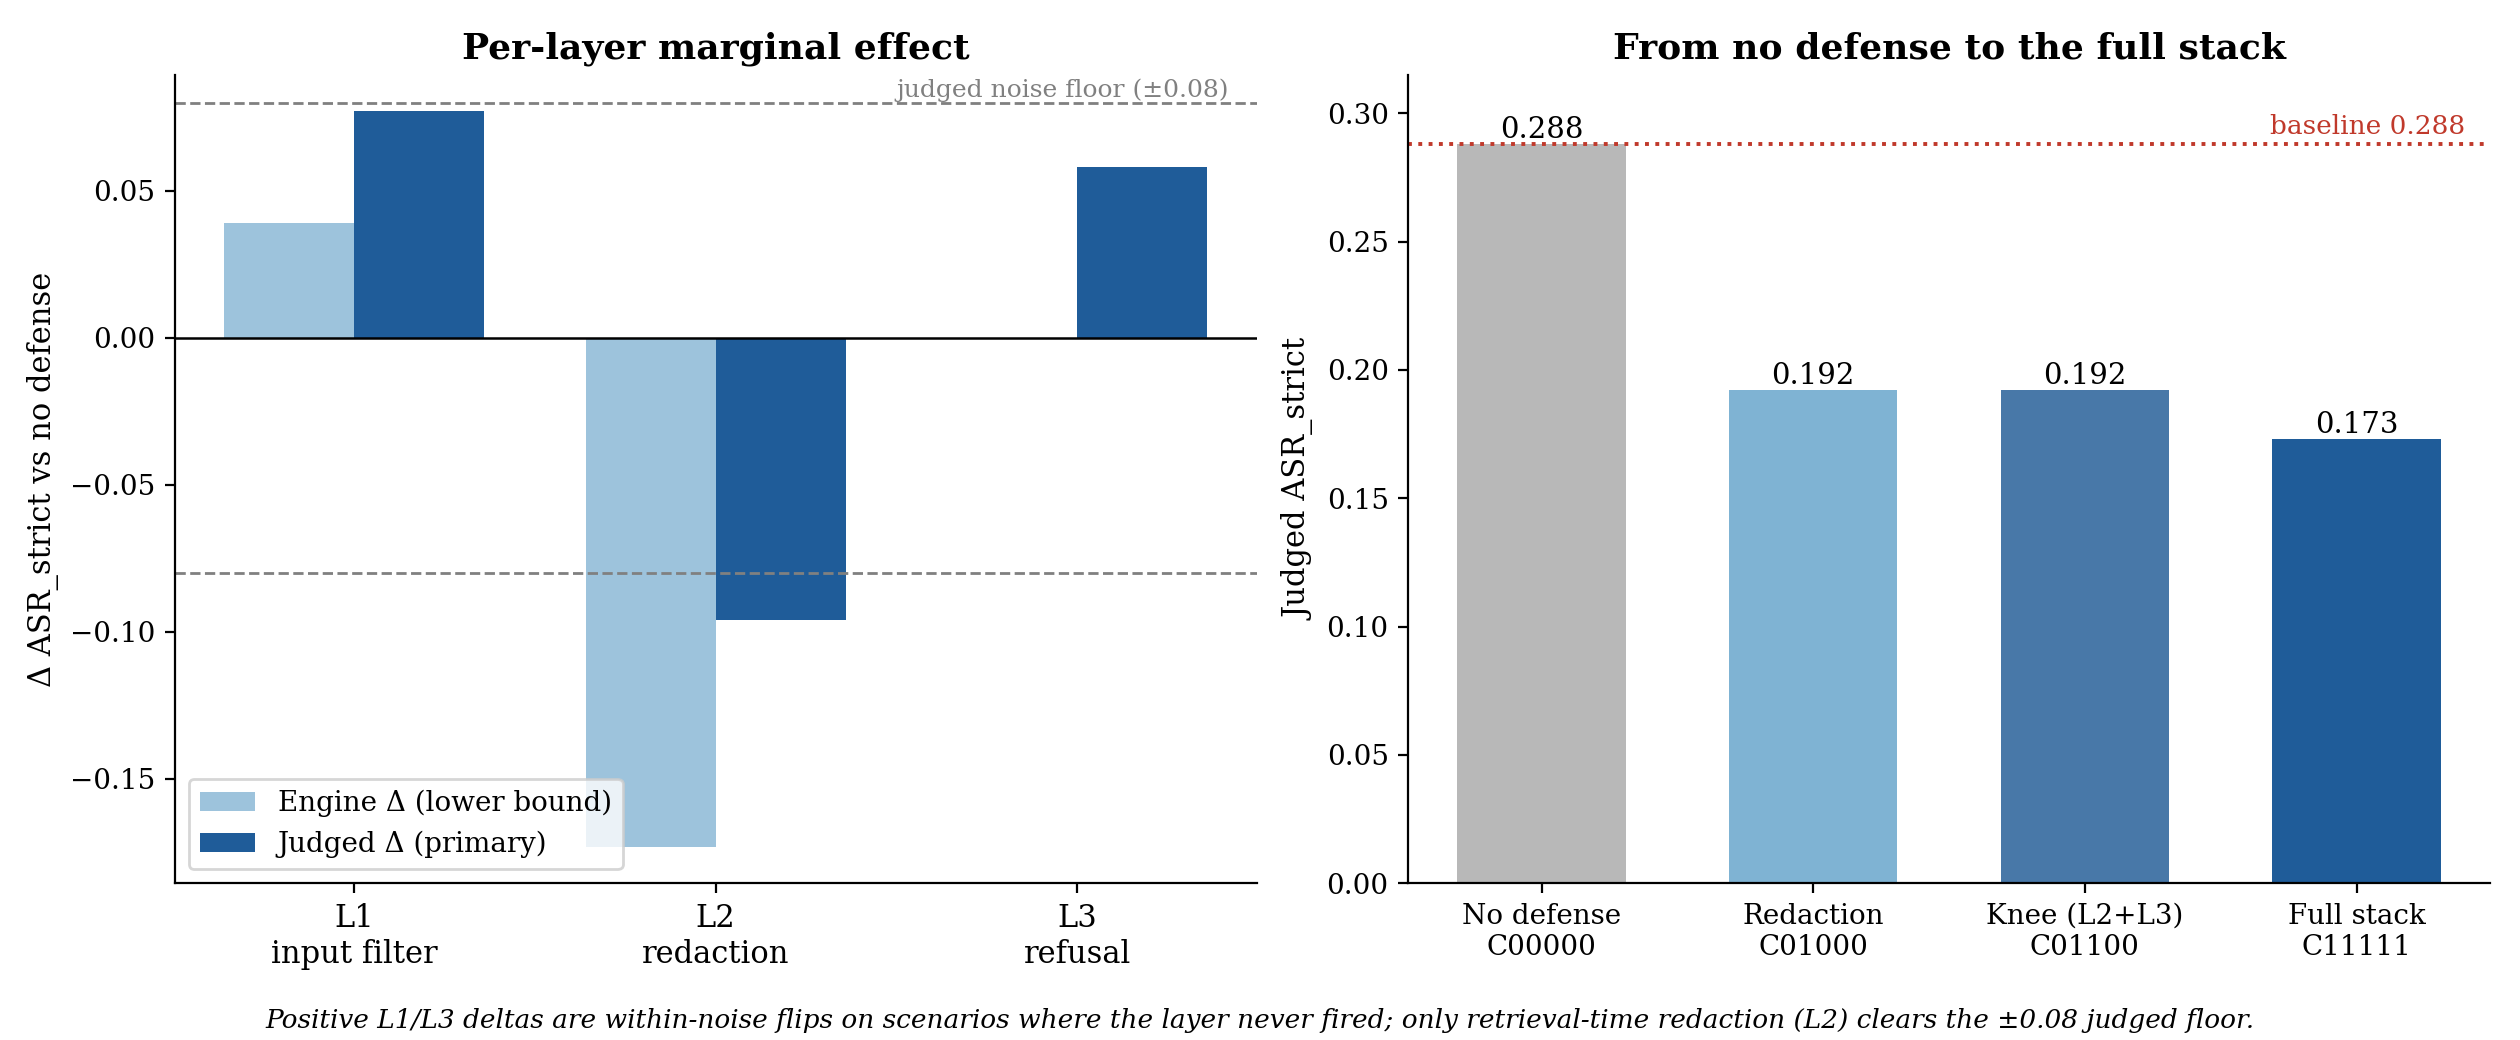
\includegraphics[width=0.94\textwidth]{fig_ch5_marginal_rq2}
\caption{Per-layer marginal effect against the judged noise floor (left), and the staircase
from no defense through redaction, the recommended pair, and the full stack (right). Only
retrieval-time redaction clears the floor.}
\label{fig:ch5-marginal}
\end{figure}

A final feature of Table~\ref{tab:ch5-headline} previews the chapter's deeper result. The
defense does not reduce every kind of leakage equally. Read by attack family, direct-PII
extraction collapses under redaction, its judged rate falling from $0.778$ at baseline to
$0.222$, while cross-document linkability does not: its judged rate moves from $0.6$ at
baseline to $0.6$ under the full stack, a change of zero. Redaction removes the entities a
detector can name; it cannot stop a model from re-associating a person out of facts that are
individually innocuous. That asymmetry is where the two instruments part company.

\section{The disagreement as the methodological headline}
\label{sec:ch5-disagreement}

Read through the rule engine alone, the defense looks total: leakage falls from $0.192$ to
$0.000$, an apparent near-elimination. Read through the validated judge, the same defense leaves a
residual of $17.3\%$. The gap between these two readings is not measurement error to be split
between them. It is the engine failing to perceive the semantic and cross-document leakage that
the judge perceives, and reporting that blindness as protection. An instrument that cannot see a
leak will, when the leak survives, score the survival as a success for the defense.

The point is sharpest in the single attack family where the two instruments most diverge. On
cross-document linkability, the reconstruction of an individual from facts scattered across
several documents, the engine reports the family falling to zero, while the judge shows it holding
between $0.6$ and $0.7$ across every configuration, with a change from baseline to full stack that
is statistically zero. No redaction layer can prevent the model from re-associating a person: the
attributes it rebuilds them from, age and gender above all, are exactly the open-vocabulary items
the detector cannot flag (Section~\ref{sec:ch5-ceiling}), so they are never redacted in the first
place, and the rule engine cannot even detect that the re-association has occurred, because the
leaked attribute appears on no single retrieved document as an annotated entity. On the family
where the engine is blindest, it most overstates the fix; a single engine-only number would have
been not just incomplete but misleading (\Cref{fig:ch5-kappa}).

\begin{figure}[h]
\centering
\begin{tikzpicture}
\begin{axis}[
  ybar, width=0.9\textwidth, height=7.2cm,
  ymin=-0.27, ymax=1.08, ylabel={Cohen's $\kappa$ vs.\ human annotation}, ylabel style={font=\small},
  xtick={1,2,3}, xticklabels={Engine\\\footnotesize linkage family,Judge\\\footnotesize undefended,Judge\\\footnotesize defended},
  x tick label style={align=center, font=\small},
  ytick={-0.2,0,0.2,0.4,0.6,0.8,1.0}, ymajorgrids, grid style={gray!15,thin},
  enlarge x limits=0.3, axis line style={gray!55}, tick style={gray!55},
]
\draw[dashed, gray!60, semithick] (axis cs:0.4,0) -- (axis cs:3.6,0);
\node[font=\scriptsize, text=gray!55!black, anchor=south west] at (axis cs:0.42,0.015) {chance ($\kappa{=}0$)};
\draw[dashed, figgreen!70!black, semithick] (axis cs:0.4,0.6) -- (axis cs:3.6,0.6);
\node[font=\scriptsize, text=figgreen!42!black, anchor=south west] at (axis cs:0.42,0.615) {gate ($\kappa{\geq}0.6$)};
\addplot+[ybar, bar width=38pt, bar shift=0pt, fill=figcoral, draw=figcoral!60!black,
  nodes near coords={$-0.10$}, every node near coord/.append style={font=\footnotesize\bfseries, anchor=north, yshift=-3pt, text=figcoral!55!black}] coordinates {(1,-0.10)};
\addplot+[ybar, bar width=38pt, bar shift=0pt, fill=figteal, draw=figteal!60!black,
  nodes near coords={$0.827$}, every node near coord/.append style={font=\footnotesize\bfseries, text=figteal!40!black}] coordinates {(2,0.827)};
\addplot+[ybar, bar width=38pt, bar shift=0pt, fill=figamber, draw=figamber!65!black,
  nodes near coords={$0.306$}, every node near coord/.append style={font=\footnotesize\bfseries, text=figorange!65!black}] coordinates {(3,0.306)};
\end{axis}
\end{tikzpicture}
\caption[The two-instrument finding: the engine is blind to linkage; the judge degrades on the
defended distribution]{The two-instrument finding. The deterministic engine's agreement with the
human annotator on the linkage family is $\kappa=-0.10$ --- no better than chance --- so it is
structurally blind to re-identification by linkage. The validated judge agrees at $\kappa=0.827$
on undefended output but degrades to $\kappa=0.306$ on the defended distribution. All three
values are measured; none is estimated.}
\label{fig:ch5-kappa}
\end{figure}

\section{Validating the judge, and the panel that was abandoned}
\label{sec:ch5-validate}

\begin{figure}[h]
\centering
\includegraphics[width=0.9\textwidth]{fig4_kappa_heatmap}
\caption[Cohen's $\kappa$ across labeller pairs and label dimensions]{Cohen's $\kappa$ across
labeller pairs (Engine--Human, Judge--Human, Engine--Judge) and label dimensions (binary,
categorical, severity) on the 46-record calibration sample. Judge--Human binary $\kappa=0.827$
(almost perfect) passes the calibration threshold $\kappa\geq0.60$; Engine--Human binary
$\kappa=0.164$ (poor) validates the engine's false-positive tendency on severity-2 refusal turns.}
\label{fig:ch5-kappa-heatmap}
\end{figure}

If the judge is to be the primary instrument, its trustworthiness has to be established
rather than assumed (\Cref{fig:ch5-kappa-heatmap}), which is the substance of RQ3. The original design called for a
multi-agent panel: an Attacker agent, a Defender agent, and an Arbitrator that would
adjudicate disagreements between judges drawn from different model families. That design was
abandoned during implementation, and the reason is itself a finding worth stating plainly.
The arbitrator, to break a tie between the primary judge and a second opinion, must be at
least as reliable as the judges it arbitrates; but drawing it from the same model family as
the primary judge makes the escalation circular: the tie-breaker shares the very biases
whose disagreement triggered the escalation, so it cannot, even in principle, improve on the
primary judge alone. Multi-agent judging panels promise independence and, when their members
share a lineage, deliver only the appearance of it. The honest resolution is a single
validated judge whose reliability is established directly against human annotation and
\emph{corroborated} across vendors, rather than a panel that manufactures the look of
consensus without its substance.

Establishing that reliability rests on a chain of inter-rater agreement statistics, measured
on the calibration set and reported with their roles kept rigorously distinct
(Table~\ref{tab:ch5-kappa}). The figure that matters, the \emph{validation}, is the
agreement between the judge and the primary human annotator, Cohen's $\kappa = 0.827$. That
this exceeds the inter-human agreement of $\kappa = 0.692$ (the agreement between the two human
annotators with each other) shows the judge to track the primary human reference at least as
closely as the second annotator does, rather than diverging idiosyncratically. The comparison
should not be over-read: agreeing with one annotator more closely than the two annotators
agree with each other is consistent with the judge being a faithful instrument, but it is
equally consistent with the judge sharing a systematic tendency with the primary annotator
that the second annotator does not. What the figure establishes is consistency with the human
reference, not superiority to human judgment. The cross-vendor figure, $\kappa = 0.843$ between
the primary judge and an independent judge from a different vendor, is \emph{corroboration},
not validation; it establishes only that the verdicts are not an artifact of one vendor's
idiosyncrasy, and it must never be cited as if it were a second human validation. On
undefended output, the judge's measured false-positive rate is $0.083$. The agreement
statistics themselves serve as the calibration evidence RQ3 asks for; no separate calibration
curve was estimated, and none is claimed.

\begin{table}[h]
\centering
\caption{The inter-rater agreement chain on the undefended calibration set, with each
figure's role.}
\label{tab:ch5-kappa}
\begin{tabularx}{\textwidth}{lcX}
\toprule
\textbf{Comparison} & \textbf{Cohen's $\kappa$} & \textbf{Role}\\
\midrule
Judge vs.\ primary human & \textbf{0.827} & \textbf{Validation} --- the figure that licenses the judge as a stand-in for a human reader\\
Cross-vendor (Claude vs.\ gpt-oss) & 0.843 & Corroboration --- not a human validation\\
Independent vendor vs.\ human & 0.777 & Second vendor against the human reference\\
Judge vs.\ second human annotator & 0.775 & Judge above the second annotator too\\
Inter-human (annotator 2 vs.\ primary) & 0.692 & The human agreement ceiling the judge exceeds\\
\bottomrule
\end{tabularx}
\end{table}

These figures, however, were all measured on \emph{undefended} output: raw model
disclosures, where a leak is explicit and easy to recognize. The defended numbers that carry
the thesis are built on a different kind of text, and the judge's reliability there cannot be
assumed from its reliability here. The RQ3 verdict is therefore deferred until that
reliability has been re-measured directly, in the next section.

\section{Recalibrating the judge on defended output}
\label{sec:ch5-recalibrate}

The defenses change what the judge is asked to read. Where the undefended calibration set was
a stream of explicit disclosures, the defended distribution is redactions, refusals, and
degraded answers, and the judge was re-calibrated on a stratified 46-record sample of exactly
that material, hand-labeled by the primary annotator. Agreement falls, and the honest way to
report the fall is to lead with the prevalence-independent measure. Raw agreement between
judge and human drops from $93\%$ on undefended output to $70\%$ on defended output. Cohen's
$\kappa$ falls further, from $0.827$ to $0.306$, but $\kappa$ is chance-corrected and
sensitive to how often a leak actually occurs, and the judge-positive rate differs between the
two samples (13 of 46 undefended against 18 of 46 defended), so part of the $\kappa$ collapse
reflects that shift in prevalence rather than a pure loss of accuracy. Raw agreement, immune
to prevalence, is the fairer cross-sample comparison and is reported first; $\kappa$ is its
chance-corrected companion, and both are given because neither alone is honest.

The errors run in both directions (Table~\ref{tab:ch5-confusion}). Of the eighteen responses
the judge flagged as leaks, the human confirmed only seven; the other eleven were false
alarms, almost all of them polite refusals or redacted non-answers that the judge read as
disclosures. In the opposite direction, of the ten leaks the human identified, the judge
missed three, each an age-bracket re-identification assembled across several dialogue turns.
Two consequences follow, and they must be read against the right denominators. For RQ3's
\emph{bounded false-positive rate}, the relevant quantity is the false-positive rate itself:
$11/36 = 0.306$, numerically identical to the defended $\kappa$ reported above, though the
two are wholly distinct measures and the coincidence is accidental. It rises from $0.083$ on
undefended output to $0.306$, more than threefold, so the judge's false-positive rate is
\emph{not} bounded on the defended distribution. Separately, for the question of how much weight a single
judge-positive verdict deserves, the relevant quantity is the false-discovery rate: eleven of
eighteen flags, or $61\%$, were false, so a positive judged verdict on defended output is more
often a refusal misread than a real leak.

\begin{table}[h]
\centering
\caption{Judge-versus-human confusion matrix on the defended calibration sample ($n=46$).}
\label{tab:ch5-confusion}
\begin{tabular}{lccc}
\toprule
 & \textbf{Human: leak} & \textbf{Human: no leak} & \textbf{Total}\\
\midrule
Judge: leak    & 7  & 11 & 18\\
Judge: no leak & 3  & 25 & 28\\
\midrule
Total          & 10 & 36 & 46\\
\bottomrule
\end{tabular}
\end{table}

The three missed leaks deserve particular attention, because they cut the opposite way from
how a missed leak usually reads. All three are cross-document re-identification by
linkage: the very family that Section~\ref{sec:ch5-disagreement} identified as the principal
unreduced residual, and that the human annotator caught. This has two implications. The
residual the thesis treats as its central finding is therefore corroborated by human
judgment, not an artifact of the judge inventing leaks where none exist. And because the
judge \emph{under-}counts that family rather than over-counting it, the $17.3\%$ residual is a
lower bound on what the instruments can see, not an upper one. The leaks that survive the
defense are, if anything, slightly more numerous than the judge reports; the missed leaks
reinforce the linkability finding rather than undermining it. On the same defended sample the
rule engine agrees with the human at $\kappa = -0.10$, no better than chance, which is why,
for all its degradation, the judge remains the instrument read as primary.

The integrated answer to RQ3 follows directly. The judge is validated against human
annotation and corroborated across vendors on undefended output, where its false-positive
rate is bounded at $0.083$; on the defended distribution that the headline numbers are
actually built from, its agreement with the human falls to $\kappa = 0.306$ and its
false-positive rate rises to roughly $31\%$, so RQ3's bounded-false-positive criterion holds
only \emph{off} the defended distribution. The judge nonetheless remains the primary
instrument on defended output, for two reasons that survive its degradation: the only
alternative instrument is below chance there, and the judge's errors are characterized rather
than unknown: over-flagging refusals in a way that inflates the apparent residual, and
under-detecting the linkage leaks that human judgment confirms are real.

\section{Honest uncertainty bounds on the residual}
\label{sec:ch5-bounds}

Because the judge's two error rates are now measured, it is tempting to use them to correct
the $17.3\%$ residual, and the textbook tool for the job is the Rogan--Gladen estimator,
which adjusts an observed rate by the instrument's sensitivity and specificity. Applied here
it returns $-34\%$, a negative leakage rate, which is impossible. The degeneracy is
diagnostic rather than fatal. The calibration sample was deliberately enriched for
judge-positives: it took \emph{all} eighteen of the judge's flagged responses but only a
fraction of its negatives, so the sample's specificity is biased low, the implied
false-positive rate exceeds the apparent leakage rate, and the estimator is driven below
zero. Sensitivity and specificity simply do not transfer from a sample stratified on the
instrument's own verdict.

The quantities that \emph{do} survive that sampling design are the positive predictive value,
estimated on the census of all eighteen positives, and the false-omission rate. The valid
estimator under verdict-stratified sampling is therefore
\[
  p \;=\; \mathrm{PPV}\cdot q \;+\; \mathrm{FOR}\cdot(1-q)
    \;=\; 0.389 \times 0.173 \;+\; 0.107 \times 0.827
    \;=\; 0.067 + 0.089 \;=\; 0.156,
\]
where $q = 0.173$ is the judged residual. The structure of the calculation is its lesson: the
first term corrects \emph{downward} for over-flagging, pulling the rate toward $6.7\%$ if one
trusted only the human-confirmed flags; the second term corrects \emph{upward} for the missed
leaks distributed across the large body of unflagged responses, adding roughly nine points
back. The two corrections very nearly cancel. Propagating the binomial uncertainty in the two
rates gives a standard error of $0.052$ and an approximate $95\%$ interval of
$[5.3\%,\,25.8\%]$, which comfortably contains $17.3\%$; the recentring is $1.7$ percentage
points, about a third of one standard error, and so unresolvable in direction.

The interval is wide on purpose. It rests on eighteen flagged and ten human-confirmed
responses, with only three misses among them (three data points), so the per-rate estimates
are imprecise by construction, and the bound should be read as honest bracketing rather than a
new precise estimate. One claim must never be made from it: that the true leakage rate lies
\emph{below} $17.3\%$. The sample was enriched for the judge's positives, which makes the
over-flagging vivid while leaving the missed leaks among the unexamined negatives easy to
under-count; the visible over-flagging tempts a ``really it is only $7\%$'' reading that
silently discards the upward correction. Moreover, all three missed leaks fall in the single
calibration stratum the sample under-drew, so reweighting the strata to their population sizes
moves the center \emph{toward} $17.3\%$, not away from it. The propagated calibration error
widens the interval around the residual; it does not lower it. The $17.3\%$ figure stands as
the residual of record, now bounded rather than overturned.

\section{Summary}
\label{sec:ch5-summary}

This chapter answered the two empirical questions at the heart of the thesis and, in doing
so, established the methodological result that frames everything after it. On \textbf{RQ2},
the full defense stack reduces judged leakage from $28.8\%$ to $17.3\%$, a genuine reduction
of roughly forty percent, carried almost entirely by retrieval-time redaction, with the
redaction-plus-refusal pair already capturing essentially all of the measurable benefit and
the further layers adding nothing the instrument can distinguish from noise. The reduction is
real but partial: direct-PII extraction collapses, while cross-document linkability survives
unreduced. On \textbf{RQ3}, a single language-model judge, validated against human annotation
at $\kappa = 0.827$, above the inter-human ceiling, and corroborated across vendors at
$\kappa = 0.843$, is a trustworthy instrument on undefended output, but its reliability
degrades on the defended distribution the headline rests on, where $\kappa$ falls to $0.306$
and its false-positive rate rises to roughly $31\%$; the originally planned multi-agent panel
was abandoned as circular, and that abandonment is itself a contribution to the LLM-as-judge
literature. The judge remains primary because the only alternative is below chance and its
errors are characterized.

The deeper result is that these two answers are entangled. The rule engine reports the
defense as near-total; the validated judge reports a $17.3\%$ residual; the difference is the
engine's blindness to semantic and cross-document leakage reported as protection. Measuring a
defended retrieval-augmented system with a single instrument is not conservative; it is
wrong in a direction the analyst cannot see. The honest residual is $17.3\%$, bounded by a
wide but informative interval of $[5.3\%,\,25.8\%]$ that contains it, corroborated rather than
inflated by the judge's measured errors. What this chapter demonstrates is a method for
measuring a defended system honestly; it does not certify the system as safe to deploy. The
cost of that residual in utility, the deployment trade-off at the knee, and the
severity-weighted ($\Delta S$, $\bar{S}$) and per-profile structure of what remains are the
subject of Chapter~\ref{ch:tradeoff}.

\ifdefined\ThesisMaster\else
  \end{document}
\fi
